% !TeX program = xelatex
\documentclass[a4paper,10pt]{article}

% ============================================================================
% សន្លឹកកិច្ចការសិស្ស ស-ខ្មៅ (Student Worksheet - Grade 8 Lesson 1: 5 RAT_DIV)
% បរិបទ៖ គ្មានស្លាយ LCD និងគ្មានម៉ាស៊ីនគិតលេខ — សិស្សបំពេញផ្ទាល់លើសន្លឹកកិច្ចការ ២ ទំព័រ A4
% ============================================================================
\usepackage[a4paper, left=0.85cm, right=0.85cm, top=0.70cm, bottom=0.95cm, footskip=0.48cm]{geometry}
\usepackage{amsmath, amssymb}
\usepackage{unicode-math}
\usepackage{fontspec}
\usepackage{array, colortbl}
\usepackage[table]{xcolor}
\usepackage{enumitem}
\usepackage{pifont}
\usepackage{fancyhdr}
\usepackage{lastpage}
\usepackage{tikz}
\usepackage[most]{tcolorbox}
\usetikzlibrary{calc, arrows.meta, decorations.pathreplacing, positioning, babel}

\makeatletter
\let\@expl@@@mark@update@singlecol@structures@@\relax
\makeatother

\providecommand{\NGSFindFonts}{%
  \IfFileExists{C:/Windows/Fonts/cambria.ttc}{%
    \def\NGSSysPath{C:/Windows/Fonts/}%
    \def\NGSUserPath{C:/Users/KIT/AppData/Local/Microsoft/Windows/Fonts/}%
  }{%
    \IfFileExists{./fonts/KhmerOSsiemreap.ttf}{\def\NGSSysPath{./fonts/}\def\NGSUserPath{./fonts/}}{%
    \IfFileExists{../fonts/KhmerOSsiemreap.ttf}{\def\NGSSysPath{../fonts/}\def\NGSUserPath{../fonts/}}{%
    \IfFileExists{../../fonts/KhmerOSsiemreap.ttf}{\def\NGSSysPath{../../fonts/}\def\NGSUserPath{../../fonts/}}{%
    \IfFileExists{../../../fonts/KhmerOSsiemreap.ttf}{\def\NGSSysPath{../../../fonts/}\def\NGSUserPath{../../../fonts/}}{%
    \IfFileExists{../../../../fonts/KhmerOSsiemreap.ttf}{\def\NGSSysPath{../../../../fonts/}\def\NGSUserPath{../../../../fonts/}}{%
    \IfFileExists{../../../../../fonts/KhmerOSsiemreap.ttf}{\def\NGSSysPath{../../../../../fonts/}\def\NGSUserPath{../../../../../fonts/}}{%
    \IfFileExists{../../../../../../fonts/KhmerOSsiemreap.ttf}{\def\NGSSysPath{../../../../../../fonts/}\def\NGSUserPath{../../../../../../fonts/}}{%
      \def\NGSSysPath{../../../../../../../fonts/}\def\NGSUserPath{../../../../../../../fonts/}%
    }}}}}}}%
  }%
}
\NGSFindFonts

\setmathfont[Path={\NGSSysPath}, FontIndex=1, Scale=1.02]{cambria.ttc}
\defaultfontfeatures{Ligatures=TeX}

\setmainfont[
  Path={\NGSUserPath}, Extension=.ttf, Script=Khmer,
  BoldFont={KhmerOSsiemreap}, BoldFeatures={FakeBold=1.8},
  ItalicFont={KhmerOSsiemreap}, ItalicFeatures={FakeSlant=0.22}
]{KhmerOSsiemreap}

\newfontfamily\muol[Path={\NGSUserPath}, Extension=.ttf, Script=Khmer]{KhmerOSmuollight}
\newfontfamily\TimesEn[Path={\NGSSysPath}, Extension=.ttf, BoldFont={timesbd}, ItalicFont={timesi}]{times}

\XeTeXlinebreaklocale "km"
\XeTeXlinebreakskip = 0pt plus 1pt minus 0.1pt

\definecolor{panelgray}{gray}{0.93}
\definecolor{headgray}{gray}{0.85}

\pagestyle{fancy}
\fancyhf{}
\renewcommand{\headrulewidth}{0pt}
\fancyfoot[L]{\fontsize{7.5pt}{9.5pt}\selectfont អនុវិទ្យាល័យព្រះក្រសាំង \en{|} គណិតវិទ្យាថ្នាក់ទី៨ \en{|} មេរៀនទី១៖ ៥. ប្រមាណវិធីចែកនៃចំនួនសនិទាន (គ្រូ៖ ហុក ប៊ុនថែន)}
\fancyfoot[R]{\fontsize{7.8pt}{9.5pt}\selectfont ទំព័រ \en{\thepage/\pageref{LastPage}}}

\setlength{\parindent}{0pt}
\setlength{\parskip}{0pt}
\setlength{\tabcolsep}{3.8pt}

\newcommand{\en}[1]{{\TimesEn #1}}
\newcommand{\enbf}[1]{{\TimesEn\bfseries #1}}
\newcommand{\unit}[1]{\,\text{\en{#1}}}
\newcommand{\cnum}[1]{\mbox{\fontsize{10pt}{12pt}\selectfont\ding{\numexpr181+#1\relax}}}
\newcommand{\chkbox}{\tikz[baseline=-0.12ex]\draw[black, line width=0.8pt] (0,0) rectangle (0.24cm,0.24cm);}
\newcommand{\blank}[1][1.5cm]{\makebox[#1]{\dotfill}}
\newcommand{\secbar}[2]{%
  \begin{tcolorbox}[enhanced, sharp corners, colback=headgray, colframe=black, boxrule=0.9pt, boxsep=1pt, top=2pt, bottom=2pt, left=5pt, right=5pt, before skip=4pt, after skip=3pt]
    {\muol\fontsize{9.2pt}{13pt}\selectfont #1}\hfill{\fontsize{8pt}{11pt}\selectfont\textbf{#2}}
  \end{tcolorbox}%
}

\newcolumntype{L}[1]{>{\raggedright\arraybackslash}p{#1}}
\newcolumntype{C}[1]{>{\centering\arraybackslash}p{#1}}

\begin{document}
\fontsize{9.6pt}{14.4pt}\selectfont

% ============================================================================
% ទំព័រទី ១៖ E1 + E2 (POE 1 & POE 2) + E3 សំយោគបញ្ញត្តិ និងធនាគារហេតុផល
% ============================================================================
\begin{tcolorbox}[enhanced, sharp corners, colback=white, colframe=black, boxrule=1.0pt, boxsep=2pt, top=3pt, bottom=3pt, left=6pt, right=6pt]
  \begin{center}
    {\muol\fontsize{10.0pt}{15pt}\selectfont អនុវិទ្យាល័យព្រះក្រសាំង \enbf{--} សន្លឹកកិច្ចការសិស្ស \enbf{(}មេរៀនទី១៖ ៥\enbf{.} ប្រមាណវិធីចែកនៃចំនួនសនិទាន\enbf{)}}\\[3pt]
    {\fontsize{8.8pt}{12pt}\selectfont
    ឈ្មោះសិស្ស / ដៃគូ៖ \blank[5.2cm] \hspace{0.25cm}
    ថ្នាក់ទី៨៖ \blank[1.1cm] \hspace{0.25cm}
    ក្រុមទី៖ \blank[1.0cm] \hspace{0.25cm}
    កាលបរិច្ឆេទ៖ ២១/១១/២០២៦}
  \end{center}
\end{tcolorbox}

% --- E1 + E2 ---
\secbar{ផ្នែកទី១៖ បេសកកម្មទស្សន៍ទាយ \enbf{(E1)} និងការរុករកជាដៃគូ \enbf{(E2 -- POE 1 \& POE 2)}}{រយៈពេល ១៤ នាទី}

\begin{tcolorbox}[enhanced, sharp corners, colback=panelgray, colframe=black, boxrule=0.75pt, boxsep=1.5pt, top=2.5pt, bottom=2.5pt, left=5pt, right=5pt]
  \textbf{បេសកកម្ម \en{E1} (គូសធីក \chkbox\ មុនពិសោធន៍ — ឧទាហរណ៍ ក ទំ.១០)៖} ជាងដេរមានខ្សែបូប្រវែង $\frac{4}{5}\unit{m}$ ចង់កាត់ជាកំណាត់ប្រវែង $\frac{1}{10}\unit{m}$ ស្មើៗគ្នា ($\frac{4}{5}\div\frac{1}{10}$)៖\\[2pt]
  \begin{center}
  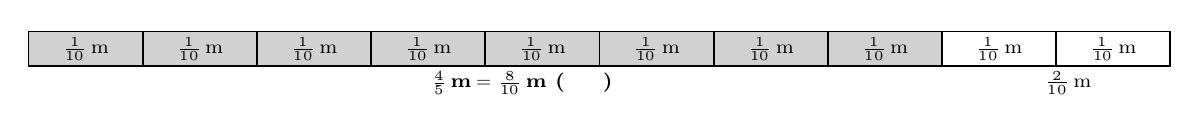
\begin{tikzpicture}[x=1.45cm, y=0.44cm, every node/.style={font=\scriptsize, text=black}]
    \foreach \i in {0,...,7} { \fill[gray!36] (\i,0) rectangle (\i+1,1); }
    \foreach \i in {0,...,9} {
      \draw[black, line width=0.65pt] (\i,0) rectangle (\i+1,1);
      \node at (\i+0.5,0.5) {$\frac{1}{10}\unit{m}$};
    }
    \node at (4.0,-0.48) {\textbf{ប្រវែងខ្សែបូ $\frac{4}{5}\unit{m} = \frac{8}{10}\unit{m}$ (ផាត់ពណ៌)}};
    \node at (9.0,-0.48) {សល់ $\frac{2}{10}\unit{m}$};
  \end{tikzpicture}
  \end{center}
  \vspace{1pt}
  (១) តើផលចែក $\frac{4}{5}\div\frac{1}{10}$ ធំជាង ឬតូចជាង $\frac{4}{5}$? \chkbox\ ធំជាង \quad \chkbox\ តូចជាង \;\en{|}\;
  (២) រាប់លើបន្ទះ៖ បានចំនួន \blank[0.9cm] កំណាត់!
\end{tcolorbox}

\vspace{3.5pt}
\textbf{ក. សកម្មភាពទី ១ (\en{POE 1})៖ សោការពារតំណាងចែក \textbf{[រក្សាទុក — គុណ — ច្រាស]} (សៀវភៅពុម្ព ទំ.១០)}

{\renewcommand{\arraystretch}{1.60}
\begin{tabular}{|L{4.80cm}|L{8.80cm}|C{4.20cm}|}
  \hline
  \rowcolor{headgray}
  \textbf{លំហាត់គោល (ទំ.១០)} & \textbf{ប្ដូរចែកជាគុណនឹងចំនួនច្រាស រួចសម្រួលខ្វែងដោយដៃ} & \textbf{ផលចែកសម្រួលរួច} \\
  \hline
  \rule[-10pt]{0pt}{26pt}១. ឧទាហរណ៍ ក៖ $\dfrac{4}{5}\div\dfrac{1}{10}$ & រក្សាទុក $\dfrac{4}{5}$ គុណច្រាសនៃ $\dfrac{1}{10}$៖ $=\dfrac{4}{5}\times\dfrac{\blank[0.7cm]}{1} = \dfrac{40}{5}$ & $\blank[1.8cm]$ \\
  \hline
  \rule[-10pt]{0pt}{26pt}២. ឧទាហរណ៍ ខ៖ $-\dfrac{3}{5}\div 2\dfrac{3}{10}$ & បំប្លែងសិន៖ $=-\dfrac{3}{5}\div\dfrac{\blank[0.7cm]}{10} = -\dfrac{3}{5}\times\dfrac{10}{\blank[0.7cm]}$ & $\blank[1.8cm]$ \\
  \hline
  \rule[-10pt]{0pt}{26pt}៣. គំរូ ខ៖ $\dfrac{28}{27}\div\dfrac{-4}{51}$ & ប្ដូរជាគុណសិន៖ $=\dfrac{28}{27}\times\dfrac{51}{\blank[0.7cm]} = \dfrac{7\times\blank[0.7cm]}{-9}$ & $\blank[1.8cm]$ \\
  \hline
  \rule[-10pt]{0pt}{26pt}៤. ចំនួនគត់ចែកប្រភាគ៖ $(-6)\div\left(-\dfrac{3}{5}\right)$ & សញ្ញាដកចែកដក $\to +$៖ $=\left(-\dfrac{6}{1}\right)\times\left(-\dfrac{\blank[0.6cm]}{3}\right)$ & $\blank[1.8cm]$ \\
  \hline
\end{tabular}}

\vspace{4pt}
\textbf{ខ. សកម្មភាពទី ២ (\en{POE 2})៖ អន្ទាក់សម្រួលខ្វែងលើសញ្ញា $\div$ — ចាប់កំហុស និងកែតម្រូវ (គំរូ ក ទំ.១០)}

\begin{tcolorbox}[enhanced, sharp corners, colback=white, colframe=black, boxrule=0.7pt, boxsep=2pt, top=2.5pt, bottom=2.5pt, left=5pt, right=5pt]
  សិស្សម្នាក់គណនា $\dfrac{24}{-25}\div\dfrac{6}{15}$ ដោយសម្រួលខ្វែងភ្លាម៖ $\dfrac{24\div 3}{-25\div 5}\div\dfrac{6\div 3}{15\div 5} \implies \dfrac{8}{-5}\div\dfrac{2}{3}$ រួចសរសេរចម្លើយ $-\dfrac{16}{15}$ (\ding{55})៖\\[3pt]
  $\bullet$ \textbf{កែតម្រូវតាមក្បួន \cnum{1}, \cnum{2}៖} $\dfrac{24}{-25}\div\dfrac{6}{15} = \dfrac{24}{-25}\times\dfrac{\blank[0.7cm]}{6} = \dfrac{4\times\blank[0.6cm]}{-5\times 1} = \blank[1.3cm]$ (\textbf{ប្ដូរជាគុណសិន ទើបសម្រួលខ្វែង!})
\end{tcolorbox}

% --- E3 ---
\secbar{ផ្នែកទី២៖ សំយោគបញ្ញត្តិ \enbf{(E3)} និងធនាគារហេតុផល \enbf{B\&W} \cnum{1}\enbf{--}\cnum{5}}{សៀវភៅពុម្ព ទំ.១០}

\begin{tabular}{|L{9.20cm}|L{9.20cm}|}
  \hline
  \textbf{១. រូបមន្តប្រមាណវិធីចែក និងការសម្គាល់សំខាន់ៗ (ទំ.១០)៖}\par\vspace{2.5pt}
  $\bullet$ \textbf{ជាទូទៅ៖} ចំពោះ $b\neq 0,\; c\neq 0,\; d\neq 0$ គេបាន៖\par\vspace{2pt}
  \hspace*{0.4cm}$\dfrac{a}{b}\div\dfrac{c}{d} = \dfrac{a}{b}\times\dfrac{\blank[0.7cm]}{\blank[0.7cm]} = \dfrac{\blank[0.9cm]}{bc}$\par\vspace{2.5pt}
  $\bullet$ \textbf{ក្បួនសញ្ញា៖} សញ្ញាដូចគ្នា $\to \blank[0.6cm]$ \;;\; សញ្ញាផ្ទុយគ្នា $\to \blank[0.6cm]$\par\vspace{2.5pt}
  $\bullet$ \textbf{ប្រយ័ត្ន៖} \textbf{ហាម}ចែកនឹង $0$ ហើយវិធីចែក\textbf{គ្មាន}លក្ខណៈត្រឡប់ទេ!
  &
  \textbf{២. ធនាគារហេតុផល \en{B\&W} (\cnum{1}--\cnum{5})៖}\par\vspace{2.5pt}
  \cnum{1} ក្បួន \textbf{[រក្សាទុក — គុណ — ច្រាស]}៖ $\frac{a}{b}\div\frac{c}{d}=\frac{a}{b}\times\frac{d}{c}$ ។\par\vspace{2.5pt}
  \cnum{2} \textbf{ហាម}សម្រួលខ្វែងលើសញ្ញា $\div$ ត្រូវប្ដូរជាគុណសិន ។\par\vspace{2.5pt}
  \cnum{3} ក្បួនសញ្ញាផលចែកដូចវិធីគុណ៖ ដូចគ្នា $\to +$ ; ផ្ទុយគ្នា $\to -$ ។\par\vspace{2.5pt}
  \cnum{4} បំប្លែងចំនួនចម្រុះជាប្រភាគ ឬរំកិលក្បៀសបំបាត់ទសភាគនៅតួចែក ។\par\vspace{2.5pt}
  \cnum{5} អាទិភាព៖ គណនាក្នុងវង់ក្រចកសិន មុនធ្វើប្រមាណវិធីចែក ។ \\
  \hline
\end{tabular}

\vspace{4pt}
\begin{tcolorbox}[enhanced, sharp corners, colback=panelgray, colframe=black, boxrule=0.65pt, boxsep=1.5pt, top=2pt, bottom=2pt, left=5pt, right=5pt]
  \textbf{ប្រយ័ត្នអន្ទាក់៖} (១) ហាមត្រឡប់តំណាងចែកប្រភាគទី១ ($\frac{a}{b}$) ដាច់ខាត! \quad (២) $0\div\left(-\frac{3}{7}\right)=0$ ប៉ុន្តែ $\left(-\frac{3}{7}\right)\div 0$ \textbf{គ្មានន័យទេ}!
\end{tcolorbox}

\vspace{4pt}
\textbf{៣. លំហាត់ត្រួតពិនិត្យរហ័ស៖ គណនាផលចែកចំនួនសនិទានដោយដៃ}

\vspace{2.5pt}
{\renewcommand{\arraystretch}{1.62}
\begin{tabular}{|C{4.40cm}|C{4.40cm}|C{4.40cm}|C{4.40cm}|}
  \hline
  \rowcolor{panelgray}
  $\frac{2}{3}\div\frac{2}{9} = \blank[1.1cm]$ & $\left(-\frac{3}{5}\right)\div\left(-\frac{3}{5}\right) = \blank[0.9cm]$ & $4\div\frac{1}{2} = \blank[1.1cm]$ & $0\div\left(-\frac{5}{8}\right) = \blank[1.0cm]$ \\
  \hline
  $\left(-\frac{4}{7}\right)\div\frac{8}{7} = \blank[1.0cm]$ & $\frac{5}{6}\div(-5) = \blank[1.0cm]$ & $-6\div\left(-\frac{2}{3}\right) = \blank[1.0cm]$ & $3.6\div(-0.9) = \blank[1.0cm]$ \\
  \hline
  $\frac{1}{4}\div 0.25 = \blank[1.0cm]$ & $\left(-\frac{9}{10}\right)\div\frac{3}{-5} = \blank[0.9cm]$ & $1\div\left(-\frac{4}{9}\right) = \blank[1.0cm]$ & $1\frac{1}{2}\div\frac{3}{4} = \blank[1.0cm]$ \\
  \hline
  $\frac{7}{8}\div 1 = \blank[1.1cm]$ & $\left(-\frac{5}{12}\right)\div\frac{5}{6} = \blank[0.9cm]$ & $-2\div\frac{1}{5} = \blank[1.1cm]$ & $(-0.8)\div(-0.2) = \blank[0.9cm]$ \\
  \hline
\end{tabular}}

\newpage

% ============================================================================
% ទំព័រទី ២៖ E4 លំហាត់គំរូ + E5 ប្រតិបត្តិ & វិនិច្ឆ័យ A-D + Exit + កិច្ចការផ្ទះ
% ============================================================================
\secbar{ផ្នែកទី៣៖ ពង្រីកចំណេះដឹងលើផលចែកទសភាគ និងកន្សោមវង់ក្រចក \enbf{(E4 --} ទំ\enbf{.}១០ និងទំ\enbf{.}១២\enbf{)}}{រយៈពេល ១០ នាទី}

\textbf{លំហាត់ពង្រីកចំណេះដឹង៖} ចូរបំពេញជំហានគណនាខាងក្រោមដោយដៃ ព្រមទាំងបញ្ជាក់លេខហេតុផល \cnum{1}--\cnum{5}៖

{\renewcommand{\arraystretch}{1.56}
\begin{tabular}{|L{4.70cm}|L{9.10cm}|C{4.00cm}|}
  \hline
  \rowcolor{headgray}
  \textbf{ប្រធានលំហាត់ (ទំ.១០ និង ១២)} & \textbf{ដំណើរការគណនាដោយដៃតាមលំដាប់ប្រមាណវិធី} & \textbf{ចម្លើយ និងហេតុផល} \\
  \hline
  \textbf{១. គំរូ គ (ទំ.១០)}\par\vspace{2pt}$\dfrac{-18}{65}\div\dfrac{-6}{25}$ & សញ្ញាដកចែកដក $\to \blank[0.5cm]$៖ $=\dfrac{-18}{65}\times\dfrac{25}{\blank[0.7cm]} = \dfrac{3\times 5}{13\times 1}$ & $=\blank[1.4cm]$ (\cnum{1}, \cnum{3}) \\
  \hline
  \textbf{២. ចែកទសភាគមានសញ្ញា}\par\vspace{2pt}$14.4 \div (-0.12)$ & រំកិលក្បៀស $2$ ខ្ទង់ស្មើគ្នា៖ $=\dfrac{14.4\times 100}{-0.12\times 100} = \dfrac{\blank[0.9cm]}{-12}$ & $=\blank[1.4cm]$ (\cnum{4}) \\
  \hline
  \textbf{៣. វង់ក្រចក (ទំ.១២ \#9ឃ)}\par\vspace{2pt}$\left(\dfrac{1}{2}-\dfrac{1}{3}\right)\div\dfrac{5}{8}$ & គណនាវង់ក្រចកសិន៖ $=\left(\dfrac{3-\blank[0.6cm]}{6}\right)\div\dfrac{5}{8} = \dfrac{1}{6}\times\dfrac{\blank[0.6cm]}{5}$ & $=\blank[1.4cm]$ (\cnum{5}, \cnum{1}) \\
  \hline
  \textbf{៤. ប្រភាគលើប្រភាគ}\par\vspace{2pt}$\left(-\dfrac{9}{14}\right) \Big/ \left(\dfrac{3}{7}\right)$ & សរសេរជាសញ្ញាចែក៖ $=\left(-\dfrac{9}{14}\right)\div\dfrac{3}{7} = -\dfrac{9}{14}\times\dfrac{\blank[0.6cm]}{3}$ & $=\blank[1.4cm]$ (\cnum{1}, \cnum{2}) \\
  \hline
\end{tabular}}

\vspace{5pt}
$\bullet$ \textbf{សំណួរឆ្លុះបញ្ចាំង \en{(EIA Looking-Back)}៖} តើ $\dfrac{4}{5}\div\dfrac{1}{10}$ ស្មើនឹង $\dfrac{1}{10}\div\dfrac{4}{5}$ ដែរឬទេ? ហេតុអ្វី?\\
ចម្លើយ៖ \chkbox\ ស្មើគ្នា \quad \chkbox\ មិនស្មើគ្នា ព្រោះ $\dfrac{1}{10}\div\dfrac{4}{5} = \blank[1.2cm] \neq 8$ (វិធីចែក\textbf{គ្មាន}លក្ខណៈត្រឡប់ទេ!)

% --- E5 ---
\secbar{ផ្នែកទី៤៖ វាយតម្លៃលទ្ធផលសិក្សា \enbf{(E5 --} ប្រតិបត្តិ ទំ\enbf{.}១០ \enbf{+} វិនិច្ឆ័យ \enbf{A--D +} សំបុត្រចេញ\enbf{)}}{រយៈពេល ១០ នាទី}

\textbf{ក. លំហាត់ប្រតិបត្តិ (សៀវភៅពុម្ព ទំ.១០ — ធ្វើជាដៃគូ រួចប្ដូរសន្លឹកផ្ទៀងផ្ទាត់ \en{Pause-Review})៖}

{\renewcommand{\arraystretch}{1.50}
\begin{tabular}{|L{8.90cm}|L{8.90cm}|}
  \hline
  \textbf{១) ប្រតិបត្តិ ក និង ខ (ទំ.១០)៖}\par\vspace{2.5pt}
  $\bullet$ \textbf{ក)} $\dfrac{8}{3}\div\dfrac{-6}{5} = \dfrac{8}{3}\times\dfrac{\blank[0.7cm]}{-6} = \blank[1.5cm]$ (\cnum{1}, \cnum{3})\par\vspace{3pt}
  $\bullet$ \textbf{ខ)} $\dfrac{40}{-27}\div\dfrac{-10}{9} = \dfrac{40}{-27}\times\dfrac{\blank[0.7cm]}{-10} = \blank[1.5cm]$ (\cnum{1}, \cnum{2})
  &
  \textbf{២) ប្រតិបត្តិ គ (ទំ.១០) និងបិទ \en{E1}៖}\par\vspace{2.5pt}
  $\bullet$ \textbf{គ)} $154.63 \div 4.7 = \blank[1.4cm] \div 47 = \blank[1.4cm]$ (\cnum{4})\par\vspace{3pt}
  $\bullet$ \textbf{បិទ \en{E1}៖} $\dfrac{4}{5}\div\dfrac{1}{10} = \blank[1.1cm]$ កំណាត់ខ្សែបូ! \\
  \hline
\end{tabular}}

\vspace{5pt}
\textbf{ខ. គូសវង់ជុំវិញជម្រើសត្រឹមត្រូវតែ ១ គត់ ក្នុងចំណោម \en{A, B, C, D} រួចសរសេរលេខហេតុផល \cnum{1}--\cnum{5}៖}

{\renewcommand{\arraystretch}{1.75}
\begin{tabular}{|L{8.90cm}|L{8.90cm}|}
  \hline
  \rule[-9pt]{0pt}{24pt}\textbf{ជម្រើស \en{A}៖} $\dfrac{8}{3}\div\dfrac{-6}{5} = \dfrac{3}{8}\times\dfrac{-6}{5} = -\dfrac{9}{20}$ &
  \textbf{ជម្រើស \en{B}៖} $\dfrac{24}{-25}\div\dfrac{6}{15} = \dfrac{4}{-5}\div\dfrac{1}{3}$ \\
  \hline
  \rule[-9pt]{0pt}{24pt}\textbf{ជម្រើស \en{C}៖} $\dfrac{40}{-27}\div\dfrac{-10}{9} = -\dfrac{4}{3}$ &
  \textbf{ជម្រើស \en{D}៖} $\dfrac{40}{-27}\div\dfrac{-10}{9} = \dfrac{40}{-27}\times\dfrac{9}{-10} = +\dfrac{4}{3}$ \\
  \hline
\end{tabular}}

\vspace{5pt}
\begin{tcolorbox}[enhanced, sharp corners, colback=panelgray, colframe=black, boxrule=0.75pt, boxsep=1.5pt, top=2.5pt, bottom=2.5pt, left=5pt, right=5pt]
  \textbf{សំបុត្រចេញពីថ្នាក់ (\en{Exit Ticket} — ៦០ វិនាទី)៖} អនុវត្តក្បួន [រក្សាទុក — គុណ — ច្រាស] រួចសម្រួលខ្វែង៖\\
  $-\dfrac{14}{15} \div \left(-\dfrac{7}{10}\right) = -\dfrac{14}{15} \times \left(\blank[1.2cm]\right) = \blank[1.4cm]$ \quad (ហេតុផល៖ \blank[1.2cm])
\end{tcolorbox}

% --- កិច្ចការផ្ទះ ---
\secbar{ផ្នែកទី៥៖ កិច្ចការផ្ទះ \enbf{(}សៀវភៅពុម្ព ទំ\enbf{.}១០ និងទំ\enbf{.}១២\enbf{)} និងបណ្ដាំផ្ញើ}{ធ្វើក្នុងសៀវភៅកិច្ចការផ្ទះ}
$\bullet$ \textbf{លំហាត់ ១៖} គណនា រួចសម្រួល៖ ក) $-\dfrac{15}{28}\div\dfrac{5}{-14}$ \qquad ខ) $\left(\dfrac{1}{2}+\dfrac{1}{3}\right)\div\left(\dfrac{5}{8}-\dfrac{1}{4}\right)$ (សៀវភៅពុម្ព ទំ.១២ \#9ង)\\
$\bullet$ \textbf{លំហាត់ ២៖} ចតុកោណកែងមួយមានបរិមាត្រ $16.38\unit{cm}$ ។ រកកន្លះបរិមាត្រ $p = 16.38\div 2$ \;\en{|}\; \textbf{អានមុន៖} ចំណុច \textbf{៦. ចំណោទ} (ទំ.១០–១២) ។

\end{document}
